% App Services
\chapter{Services der Hochschul-App}
\label{sec:appservices}
%Text

Wie im vorhergehenden Kapitel \ref{sec:architektur} bereits beschrieben wurde, basiert eine Microservice Architektur darauf, dass man einzelne Funktionalitäten der Anwendung in einzelne Services aufteilt. Die allgemeinen Richtlinien bei der Erstellung einer Web Service Architektur wurden ebenfalls schon im Kapitel \ref{sec:webservices} zum Thema Web Services beschrieben. 
\\
\linebreak
Im Allgemeinen werden die Services der Datenschnittstelle der neuen Hochschul App anhand der funktionalen Anforderungen und der architekturbedingten Vorgaben aufgeteilt. Die Services für den Stundenplan, die Stundenplanänderungen, den Mensaplan, die Benachrichtigungen und der Authentifikation bilden einzelne Services, die sich nach der entsprechenden funktionalen Anforderung richten. Die Namensgebung beschreibt hier in dem Fall schon eindeutig, welche Aufgaben jeder einzelne Service erfüllt. Die eindeutige Namensgebung trifft in diesem Fall auch auf den Anwenderservice zu, welcher sich jedoch weniger nach den funktionalen Anforderungen richtet, sondern vielmehr an den technischen Vorgaben der Microservice Architektur. In diesem Fall wird eine Funktion der Anwendung so ausgelagert, dass keine der anderen Services von diesem einen Service abhängig sind. Dieser Service ermöglicht es dennoch, die Funktion der Anwenderverwaltung zu kapseln und somit redundanten Programmcode weitgehend zu vermeiden. Die genauen Anforderungen an die einzelnen Services, deren Funktionsweise und Aufbau, sowie die grundlegende Struktur der dahinter liegenden Daten werden im folgenden genauer erarbeitet.  

% Stundenplan
\section{Stundenplan (Timetable-Service)}
\label{sec:stundenplan}
% Text

Die wichtigste Funktion der Hochschul-App soll es sein, den Stundenplan leichter für mobile Endgeräte darzustellen. Wie bereits in den vorhandenen Anwendungen der Hochschule Hof baut auf dieser Funktion die komplette Anwendung auf. Demnach ist es wichtig, dass die Erarbeitung dieser zentralen funktionalen Anforderung unter höchster Sorgfalt geschieht. Diese beinhaltet nicht nur die Bereitstellung des allgemeinen Stundenplans zum Verlesungsangebot der Hochschule, sondern auch die Möglichkeit, personalisierte Anfragen an die Datenquelle zu stellen, die in einer grafischen Oberfläche ebenfalls in einen personalisierten Stundenplan umgewandelt werden können. 

% Stundenplan Anforderung
\subsection*{Anforderung an Schnittstelle}
\label{sec:stundenplan_anforderung}
% Text

Die Daten zum Vorlesungsangebot der Hochschule Hof werden separat zur Anwendung in einer Datenbank gehalten und gepflegt. Zur Nutzung dieser und zum Arbeiten mit den Daten werden diese allerdings in modifizierter Form in einer eigenen Datenbank abgelegt. Die Schnittstelle des Services muss dem Client alle relevanten Daten zu den einzelnen Vorlesungen geben. Diese Vorlesungen kann der Client einzeln oder in verschiedenen Listen abfragen. 
\\
\linebreak
Jede einzelne Vorlesung muss mindestens folgende Informationen liefern:

\begin{itemize}

\item Eine eindeutige Kennung der Vorlesung (ID)

\item Der Name der Vorlesung

\item Die Art der Vorlesung

\item Dozent der Veranstaltung

\item Start und Ende der Vorlesung (speziell für Block-/ Sonderveranstaltungen)

\item Vorlesungszeiten

\item Die Studiengänge, in denen die Vorlesung angeboten wird

\item Fachsemester der Vorlesung

\item Vorlesungsraum

\end{itemize}

Die Daten lassen sich in allgemeine Informationen zur Veranstaltung, zeitliche Einschränkungen und in Informationen zum Rahmen der Vorlesung aufteilen. Beim Abfragen der Daten muss der Client die Möglichkeit haben, eine Liste von Veranstaltungen anhand von verschiedenen Suchkriterien zu erhalten. Möchte ein möglicher Nutzer demnach seinen aktuellen Stundenplan abfragen, so muss der Client eine Anfrage stellen können, die den Studiengang und das Fachsemester enthält. Die Antwort muss dann das komplette Vorlesungsangebot für diesen Nutzer enthalten. Ähnlich verhält es sich bei Suchen nach speziellen Vorlesungen. Es muss möglich sein, eine Liste an Vorlesungen zu erhalten, die gewisse Suchkriterien erfüllen. Möchte der Client demnach eine Liste aller Vorlesungen eines Dozenten haben, oder alle Veranstaltungen zu einem gewissen Zeitpunkt abfragen, so muss er das tun, indem er diese Suchkriterien in der Anfrage angibt. 
\\
\linebreak
Anders als beim personalisierten Stundenplan gibt der Client bei einem allgemeinen Stundenplan eine Anfrage ab, bei der er nicht weiß, welche und wie viele Ergebnisse er zurückerhält. Möchte der Client allerdings die in einem personalisierten Stundenplan abgelegten Vorlesungen abfragen, so muss er eine Anfrage stellen, in der alle eindeutigen Kennzeichnungen der Vorlesungen enthalten sind. Solang eine Kennung auch existiert, muss die Schnittstelle die zugehörigen Daten auch zurückgeben.

% Stundenplan Umsetzung
\subsection*{Spezifikation der Ressourcen}
\label{sec:stundenplan_api}
% Text 

In den GET-Methoden der Subresource /room/\{room\} können im Body die Filter für Uhrzeit, Datum oder Wochentag übergeben werden. Für die restlichen Subresourcen, außer /\{id\} und /\{name\}, können Filter für Dozent, Uhrzeit, Vorlesungssprache, Art der Vorlesung und Datum oder Wochentag übergeben werden. Die Filter Parameter sind optional, ohne eine Übergabe der Filter werden standardmäßig alle Vorlesungen zurückgegeben.  

\begin{itemize}
\item \subsubsection{GET/POST/DELETE:\\ /lectures} 
Die Methode GET liefert alle Vorlesungen unter der Berücksichtigung von gesetzten Filtern. POST erlaubt erstellen von einer oder mehreren Vorlesungen und DELETE löscht alle Vorlesungen.

\item \subsubsection{GET/PATCH/DELETE:\\ /lectures/\{id\}} 
Die Methode GET liefert eine Vorlesung für die übergebende ID. Mit PATCH kann die Vorlesung geändert beziehungsweise korrigiert werden und DELETE löscht diese Vorlesung.

\item \subsubsection{GET:\\ /lectures/\{lecture\}} 
Liefert eine Vorlesung unter der Berücksichtigung von übergebenen Vorlesungsbezeichnung.
\item \subsubsection{GET/POST/DELETE:\\ /lectures/faculty} 
Die Methode GET liefert eine Liste vorhandener Fakultäten. POST erlaubt die Fakultätsliste zu erweitern und DELETE löscht die komplette Fakultätsliste.
\item \subsubsection{GET/PATCH/DELETE:\\ /lectures/faculty/\{faculty\}} 
Die Methode GET liefert alle Vorlesungen die zur der übergebende Fakultät gehören. Mit PATCH kann die Fakultät geändert beziehungsweise korrigiert werden und DELETE löscht diese Fakultät aus der Fakultätsliste.
\item \subsubsection{GET/POST/DELETE:\\ /lectures/faculty/\{faculty\}/program} 
Die Methode GET liefert eine Liste vorhandener Studiengänge. POST erlaubt die Studiengangliste zu erweitern und DELETE löscht die komplette Studiengangliste.
\item \subsubsection{GET/PATCH/DELETE:\\ /lectures/faculty/\{faculty\}/program/\{program\}} 
Die Methode GET liefert alle Vorlesungen die zur gesetzten Fakultät und Studiengang gehören. Mit PATCH kann der Studiengang geändert beziehungsweise korrigiert werden und DELETE löscht diesen Studiengang aus der Studiengangliste.
\item \subsubsection{GET/POST/DELETE:\\ /lectures/faculty/\{faculty\}/program/\{program\}/semester} 
Die Methode GET liefert eine Liste vorhandener Semester. POST erlaubt die Semesterliste zu erweitern und DELETE löscht die komplette Semesterliste.
\item \subsubsection{GET/PATCH/DELETE:\\ /lectures/faculty/\{faculty\}/program/\{course\}/program/\{semester\}} 
Die Methode GET liefert alle Vorlesung die zur der gesetzten Fakultät, Studiengang und Semester gehören. Mit PATCH kann der Semester geändert beziehungsweise korrigiert werden und DELETE löscht diesen Semester aus der Semesterliste.

\item \subsubsection{GET:\\ /lectures/room} 
Liefert eine Liste vorhandener Vorlesungsräume.
\item \subsubsection{GET:\\ /lectures/room/\{room\}} 
Liefert alle Vorlesungen die zur gesetzten Raum gehören unter der Berücksichtigung gesetzter Filterkriterien.

\item \subsubsection{GET:\\ /lectures/filters}
Liefert alle vorhandenen Filterkriterien wie Dozenten, Vorlesungssprache, Vorlesungsart, Uhrzeit, Datum und Wochentag.
\item \subsubsection{GET/POST/DELETE:\\ /lectures/filters/instructor} 
Die Methode GET liefert eine Liste aller Dozenten. Mit POST können ein oder mehrere neue Dozenten eingefügt werden und DELETE löscht die komplette Dozentenliste.
\item \subsubsection{GET/PATCH/DELETE:\\ /lectures/filters/instructor/\{id\}}
Die Methode GET liefert Informationen zur der übergebenen Dozenten ID. Mit PATCH kann die Information zum dem Dozent geändert beziehungsweise korrigiert werden und DELETE löscht diesen Dozenten.
\item \subsubsection{GET:\\ /lectures/filters/time} 
Liefert die Formatierung für den Filter Uhrzeit.
\item \subsubsection{GET/POST/DELETE:\\ /lectures/filters/language} 
Die Methode GET liefert eine Liste verfügbarer Vorlesungssprachen. Mit POST können ein oder mehrere Vorlesungssprachen eingefügt werden und DELETE löscht die komplette Vorlesungssprachenliste.
\item \subsubsection{GET/PATCH/DELETE:\\ /lectures/filters/language/\{id\}} 
Die Methode GET liefert Informationen zur der übergebenen Vorlesungssprachen ID. Mit PATCH kann die Vorlesungssprache geändert beziehungsweise korrigiert werden und DELETE löscht diese Vorlesungssprache.
\item \subsubsection{GET:\\ /lectures/filters/type} 
Liefert eine Liste vorhandener Vorlesungstypen.
\item \subsubsection{GET:\\ /lectures/filters/date} 
Liefert die Formatierung für den Filter Datum.
\item \subsubsection{GET:\\ /lectures/filters/day} 
Liefert eine Liste vorhandener Wochentagen und den Format für den Filter.
\end{itemize}

% Stundenplan DB
\subsection*{Datenbank Konzept}
\label{sec:stundenplan_db}
%Text

Wie bereits erwähnt liegt für die Stundenplan Daten und die zugehörigen Informationen zu Änderungen und Fremdschlüsseltabellen bereits eine Datenbank zur Verfügung. Diese läuft aktuell auf dem Lehre Server der Hochschule Hof. 
\\
\linebreak
Dort ist eine MySQL Installation vorzufinden, auf der die Datenbank \textit{huapp_time_\-table} liegt. Jedoch gibt es bei der original Datenbank einige Designspezifikationen, welche das Arbeiten mit dieser für die Stundenplan Funktion schwierig macht. Das ausschlaggebende Problem, welches zur Nutzung einer eigenen Datenbank geführt hat, ist die Neugenerierung der Primärschlüssel, wenn ein neuer Eintrag geschrieben wurde. Dies macht die Abfrage durch außerhalb gespeicherte IDs unsicher, da diese ID durch die Neuvergebung des Primärschlüssels eventuell nicht vergeben oder einem anderen Eintrag vergeben wurde. Deshalb liegt der Fokus der selbst entwickelten Datenbank darauf, die Einträge der Vorlesungen eindeutig zu halten, auch wenn sich eine Vorlesung dauerhaft ändert. Die Herausforderung dabei ist, dass man erkennen muss, wenn sich ein Eintrag geändert hat. 

\begin{figure}[H]
\centering
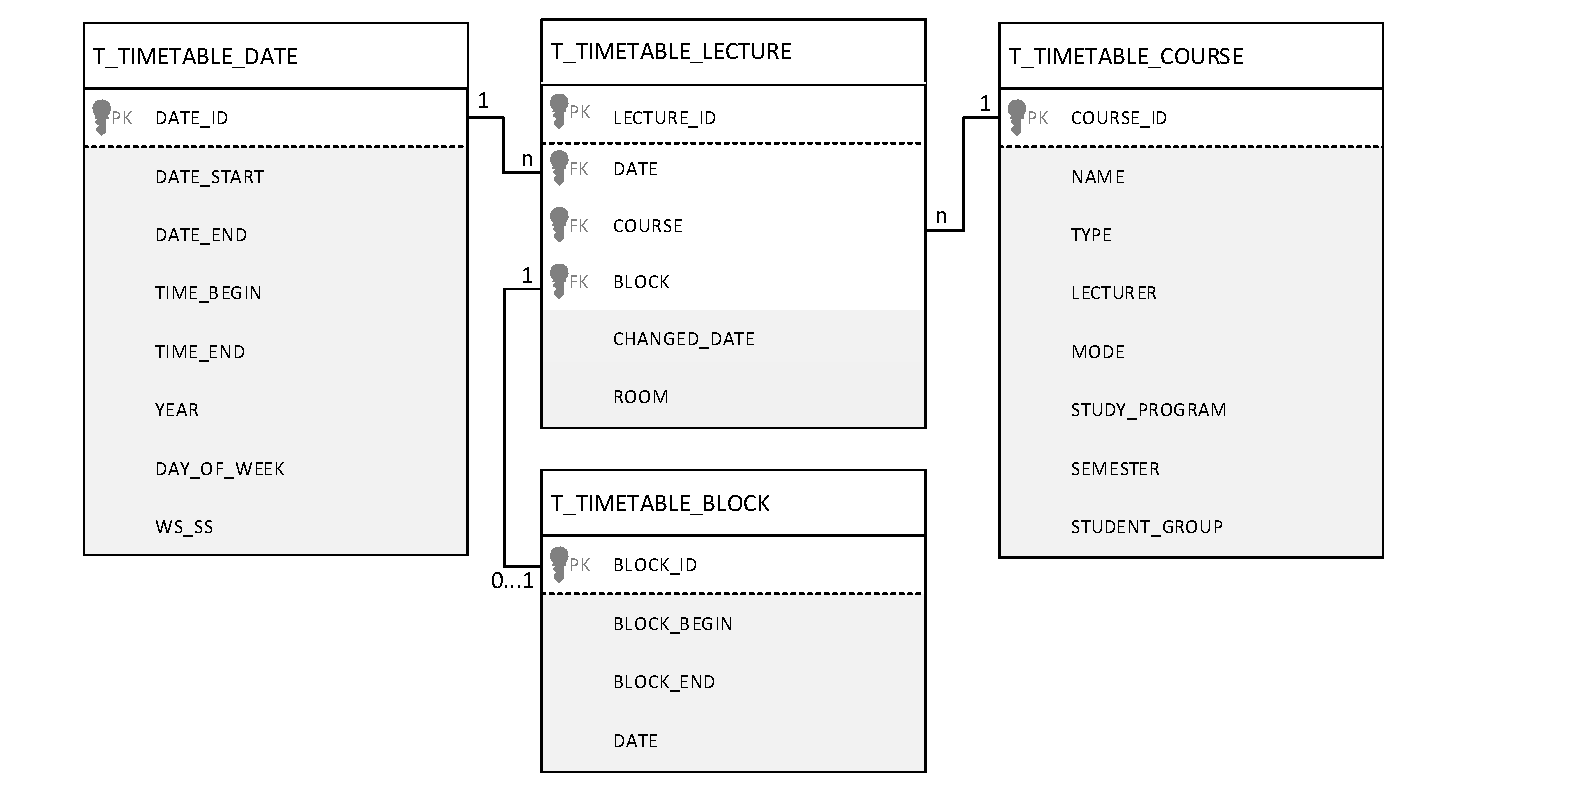
\includegraphics[width=\pictureWidth cm + 3 cm]{Bilder/ER/Timetable_ER.pdf}
\caption{Entity Relation Diagramm der Stundenplan Datenbank\label{fig:timetableER}\protect\footnotemark}
\end{figure}
\footnotetext{Brysiuk, Lehmann (2019)}


% Stundenplanänderung
\section{Planänderungen (Timetable-Change-Service)}
\label{sec:stundenplan}
% Text

Zusätzlich zu der zentralen Aufgabe des allgemeinen und personalisierten Stundenplans muss die Anwendung auch die Änderungen am Stundenplan für den Nutzer zur Verfügung stellen. Dies muss auf verschiedenen Wegen möglich sein. Die Änderungen müssen einerseits frei aufrufbar sein, das heißt, nach einer Anfrage an die Schnittstelle zurückgegeben werden, als neue Änderung aber auch von außen in die Datenquelle eingespeist werden. Um die Benachrichtigung der Clients der Schnittstelle ist dann ein anderer Service zuständig, der seine Informationen jedoch vom Stundenplanänderung-Service bezieht.
\\
\linebreak
Eine normale Anfrage an die vorhandenen Änderungen kann nochmals in zwei Arten unterteilt werden. Einerseits muss die Schnittstelle alle Daten zurückgeben können, die sie enthält, andererseits soll eine Anfrage auch gefilterte Ergebnisse zurückerhalten können. So kann ein registrierter Nutzer beispielsweise alle Änderungen abfragen, die seine Vorlesungen betreffen oder die sein Fachsemester in seinem Studiengang betreffen. 
\\
\linebreak
Die Daten, die die Anwendung auf eine solche Anfrage zurückgibt, muss mindestens folgende Informationen enthalten:

\begin{itemize}

\item Kennzeichnung der Vorlesung (Kann bei der Zuordnung zu einer echten Vorlesung genutzt werden)

\item Art der Änderung (Ausfall, Verschiebung, etc.)

\item Zeitpunkt der Änderung (Datum, Uhrzeit)

\end{itemize}

Anhand dieser Informationen ist nicht nur die allgemeine Vorlesung identifizierbar, sondern auch der Termin, an dem die Änderung eintrifft. Dies ist besonders bei Verschiebungen oder Ausfällen von einzelnen Veranstaltungen wichtig.

% Stundenplanänderung Anforderung
\subsection*{Anforderung an Schnittstelle}
\label{sec:stundenplan_change_anforderung}
% Text

Der Service und die Schnittstelle für die Stundenplanänderungen ist im Vergleich zum Stundenplan Service relativ leichtgewichtig. Hier wird lediglich eine Schnittstelle benötigt, welche die Änderungen bereitstellt. Diese sollten entweder alle ausgegeben oder anhand von Kriterien wie Datum, Studiengang oder ähnlichem gefiltert werden. Zudem soll es möglich sein, neue Änderungen über die \ac{REST}-Schnitt\-stelle hinzuzufügen, da im Hintergrund des Services eine eigene Datenbank stehen soll. Zudem muss der Service den Benachrichtigungsservice über neue Änderungen informieren, sobald er diese erkennt. 

% Stundenplanänderung Umsetzung
\subsection*{Spezifikation der Ressourcen}
\label{sec:stundenplan_change_api}
% Text
In der Ressource \lstinline[columns=fixed]{/changes} und allen Subressourcen außer \lstinline|/{id}| und \lstinline[columns=fixed]{/filters} kann im Body der Filter für das Datum übergeben werden.

\begin{itemize}
\item \subsubsection{GET/POST/DELETE:\\ /changes}
Die Methode GET liefert alle Änderungen unter der Berücksichtigung vom gesetzten Datum. POST erlaubt erstellen von eine oder mehreren Änderungen und DELETE löscht alle Änderungen.
\item \subsubsection{GET/PATCH/DELETE:\\ /changes/\{id\}} 
Die Methode GET liefert eine Änderung für die übergebene \ac{ID}. Mit PATCH kann die Vorlesung Änderung geändert beziehungsweise korrigiert werden und DELETE löscht diese Änderung
\item \subsubsection{GET/POST/DELETE:\\ /changes/program} 
Die Methode GET liefert eine Liste vorhandener Studiengänge. POST erlaubt die Studiengangliste zu erweitern und DELETE löscht die komplette Studiengangliste.
\item \subsubsection{GET/PATCH/DELETE:\\ /changes/program/\{program\}} 
Die Methode GET liefert alle Änderungen die zur gesetzten Studiengang gehören. Mit PATCH kann der Studiengang geändert beziehungsweise korrigiert werden und DELETE löscht diesen Studiengang aus der Studiengangliste.
\item \subsubsection{GET/POST/DELETE:\\ /changes/program/\{program\}/semester} 
Die Methode GET liefert eine Liste vorhandener Semester. POST erlaubt die Semesterliste zu erweitern und DELETE löscht die komplette Semesterliste.
\item \subsubsection{GET/PATCH/DELETE:\\ /changes/program/\{program\}/semester/\{semester\}} 
Die Methode GET liefert alle Änderungen die zu gesetzten Studiengang und Semester gehören. Mit PATCH kann der Semester geändert beziehungsweise korrigiert werden und DELETE löscht diesen Semester aus der Liste.
\item \subsubsection{GET:\\ /changes/filters} 
Liefert alle vorhandenen Filterkriterien, in dem Fall nur das Datum.
\item \subsubsection{GET:\\ /changes/filters/date} 
Liefert die Formatierung für den Filter Datum.
\end{itemize}

% Stundenplanänderung DB
\subsection*{Datenbank Konzept}
\label{sec:stundenplan_change_db}
%Text

Die Stundenplanänderungen liegen, wie die Stundenplaninformationen, ebenfalls bereits auf dem Lehre Server der Hochschule Hof in der Datenbank \textit{huapp_time_\-table}. Dort existiert eine Tabelle, in der die Veranstaltungen, die sich ändern, mit den alten Daten und den neuen Daten abgelegt werden. Jedoch werden diese Änderungen nur mit den Namen der dazugehörigen Vorlesung und den zeitlichen Daten der ursprünglichen Veranstaltung hinterlegt. Es wurde kein Fremdschlüssel genutzt, um die Vorlesung, die betroffen ist, mit der Änderung zu verknüpfen. Somit sind die Daten für das menschliche Auge durchaus lesbar, für Maschinen aber nur schwer zu verarbeiten.
\\
\linebreak
Deshalb wird auch hierfür eine eigene Datenbank genutzt, welche die eingehenden Einträge mit den vorhandenen Vorlesungen abgleicht und mit der passenden Vorlesungs-ID referenziert. Somit kann jede Änderung auch einer einzigen Veranstaltung zugeordnet werden. Dies erfordert jedoch einen externen Service, welcher die Tabellen der originalen Datenbank miteinander Vergleicht und daraus die Einträge für die neue Datenbank generiert. 

\begin{figure}[H]
\centering
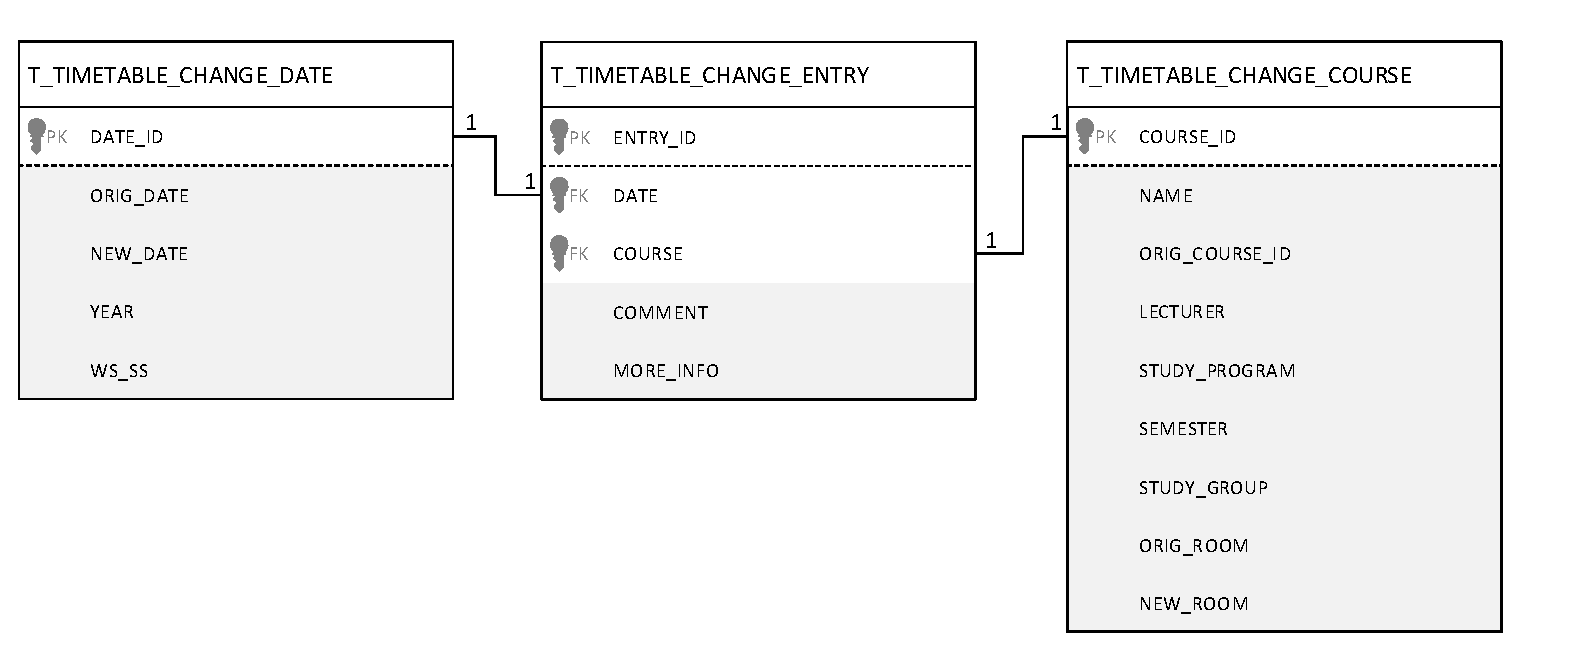
\includegraphics[width=\pictureWidth cm + 2.5 cm]{Bilder/ER/TimeTableChange_ER.pdf}
\caption{Entity Relation Diagramm der Datenbank zu den Planänderungen\label{fig:timetableER}\protect\footnotemark}
\end{figure}
\footnotetext{Brysiuk, Lehmann (2019)}

% Mensa
\section{Speiseplan (Mensa-Service)}
\label{sec:mensa}
% Text
Bei der Wahl der Ernährung spielen soziale, politische, ökonomische, psychologische und kulturelle Dimensionen eine Rolle. Somit macht die Ernährung mehr als nur den Körper mit Nährstoffen zu versorgen. 
%Referenz: https://www.dge.de/presse/pm/der-mensch-ist-was-er-isst-1/
Das Ziel ist es, den Studierenden die Möglichkeit zur Verfügung stellen, ihren Speiseplan individuell nach ihren Bedürfnissen anzupassen. Dies wird durch den Mensa-Service realisiert. Der Service stellt dem Client alle Informationen über Gerichte zur Verfügung und erlaubt auch diese gezielt zu sortieren und zu personalisieren.

% Mensa Anforderung
\subsection*{Anforderung an Schnittstelle}
\label{sec:mensa_anforderung}
% Text
Eine Schnittstelle für die Speiseplan Daten steht derzeit nicht zur Verfügung. Die Informationen für den Speiseplan, die für die Hochschul-App benötigt werden, werden auf der Webseite des Studentenwerk-Oberfranken im Navigationsmenü Speiseplan für die Standorte Hof und Münchberg zur Verfügung gestellt. Der Ausschnitt der Webseite für den Speiseplan aus Abbildung \ref{fig:swo_speiseplan} lässt sich in 7 Bereiche kategorisieren:

\begin{figure}[H]
\centering
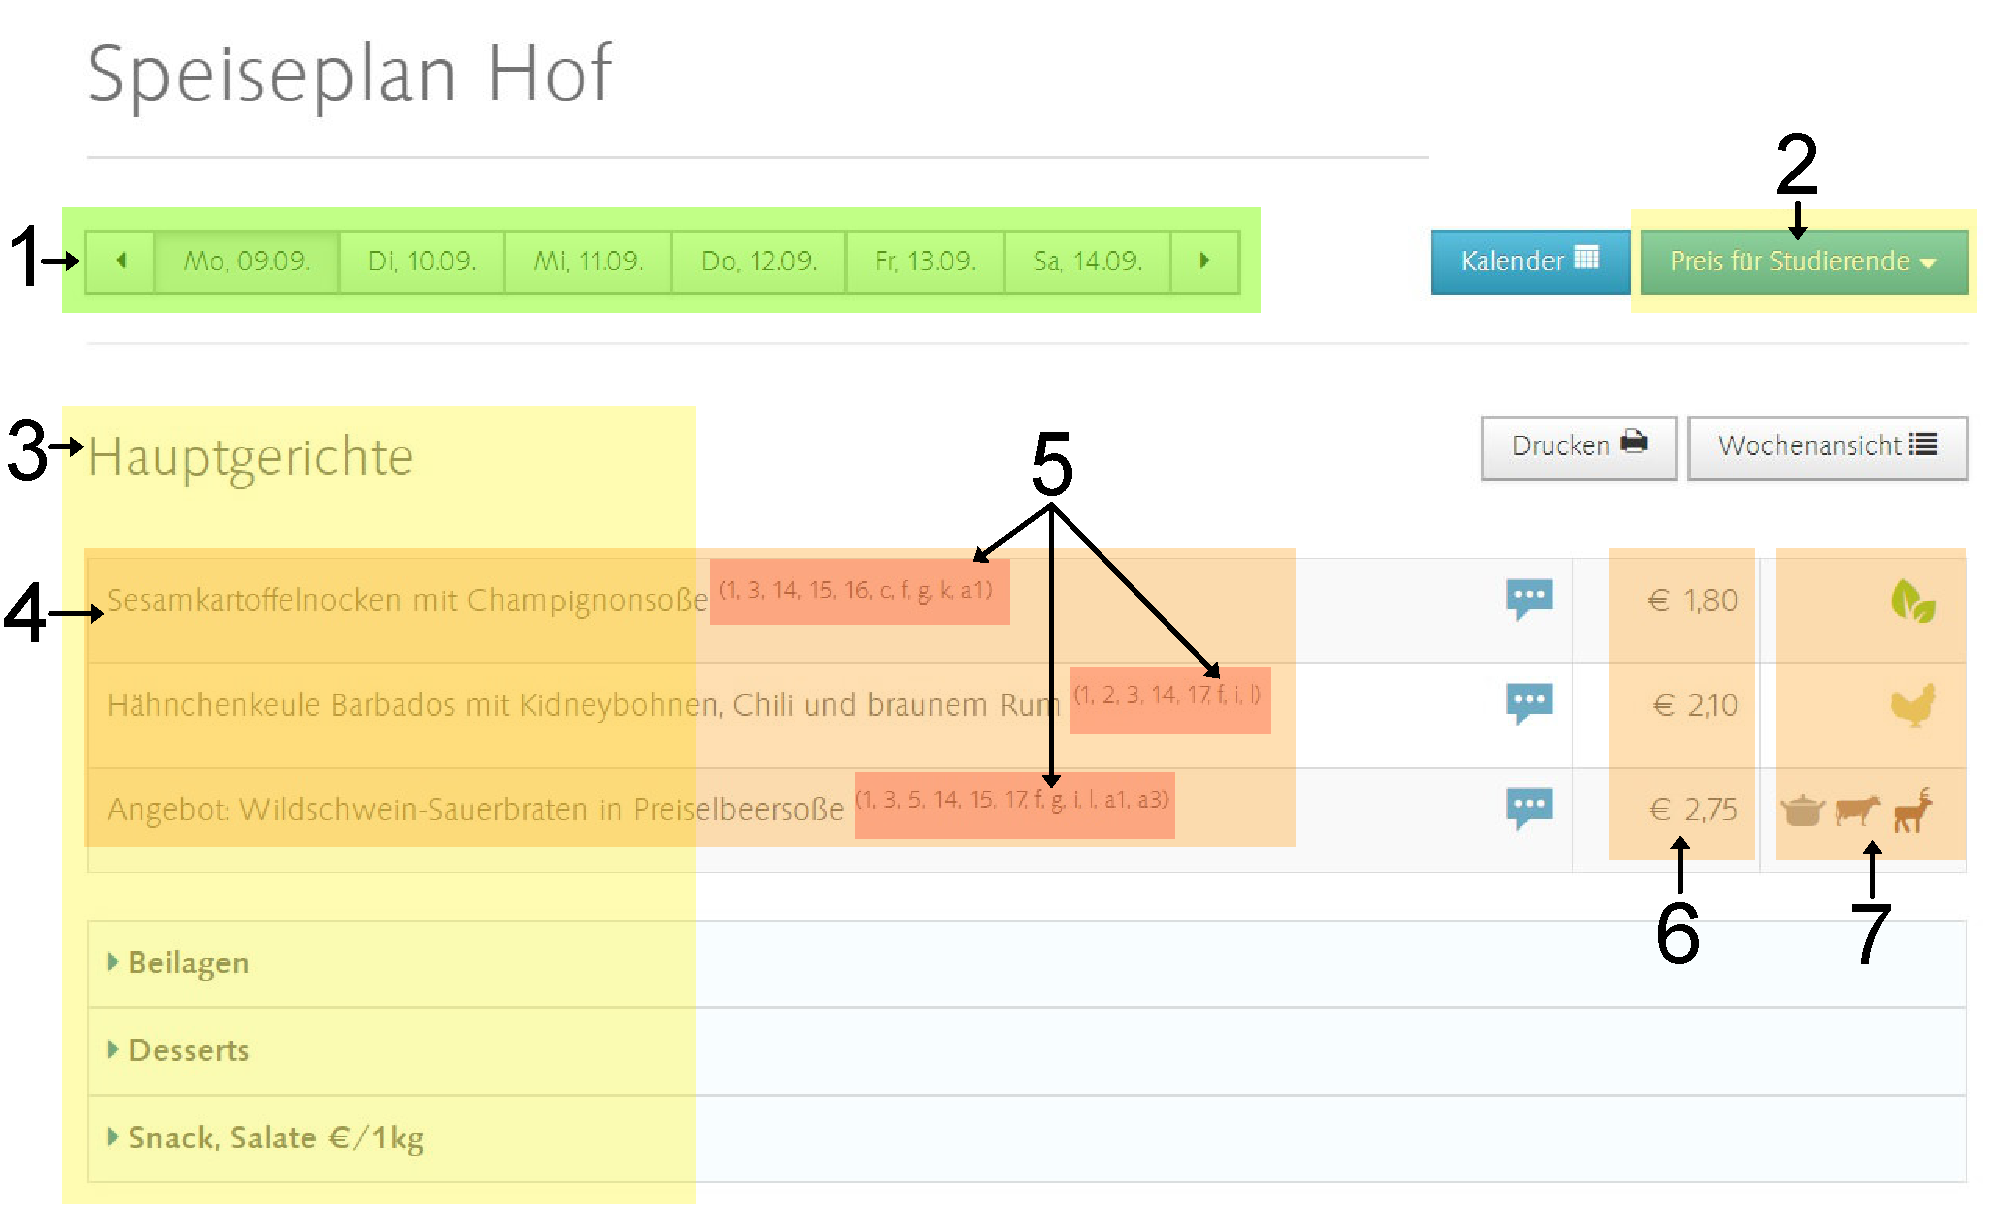
\includegraphics[width=\pictureWidth cm + 2cm]{Bilder/Sonstiges/Speiseplan_Infoblock.pdf}
\caption{Speiseplan Informationsblöcke\label{fig:swo_speiseplan}\protect\footnotemark}
\end{figure}
\footnotetext{Brysiuk, Lehmann (2019)}


\begin{enumerate}
\item Datum für Speiseplan
\item Preistyp für alle Gerichte
\item Kategorie des Gerichts
\item Bezeichnung des Gerichts
\item Zusatzstoffe/ Inhaltsstoffe/ Allergien des Gerichts
\item Preis des Gerichts
\item Kennzeichnung des Gerichts
\end{enumerate}

Wobei sich diese sieben Blöcke in drei weitere übergeordnete Bereiche einordnen lassen. Der erste bezieht sich auf die zeitliche Darstellung des Speiseplans. Der Speiseplan muss für ein beliebiges Datum oder einen Zeitraum dargestellt werden können. Der zweite bezieht sich auf die Darstellung und den Umfang des Speiseplans, bei dem der Preistyp und die Kategorie der Gerichte eine Rolle spielt. Also muss der Speiseplan zusätzlich zu den zeitlichen Einstellungen die Gerichte nach Preistyp und Kategorie sortiert werden können. Der dritte Block bezieht sich auf ein spezifisches Gericht, bei dem Bezeichnung, Zusatzstoffe/ Inhaltsstoffe/ Allergene, Kennzeichnung und der Preis des Gerichts eine Rolle spielen. Durch die Abbildung \ref{fig:analysemensa} wird dargestellt, nach welchen Faktoren der Speiseplan sortiert und personalisiert werden kann. Es muss aber beachtet werden, dass das Backend nur für Kategorisierung und Filterung der einzelnen Gerichten zuständig ist und das Frontend für die Implementierung der Suche.

\begin{figure}[H]
\centering
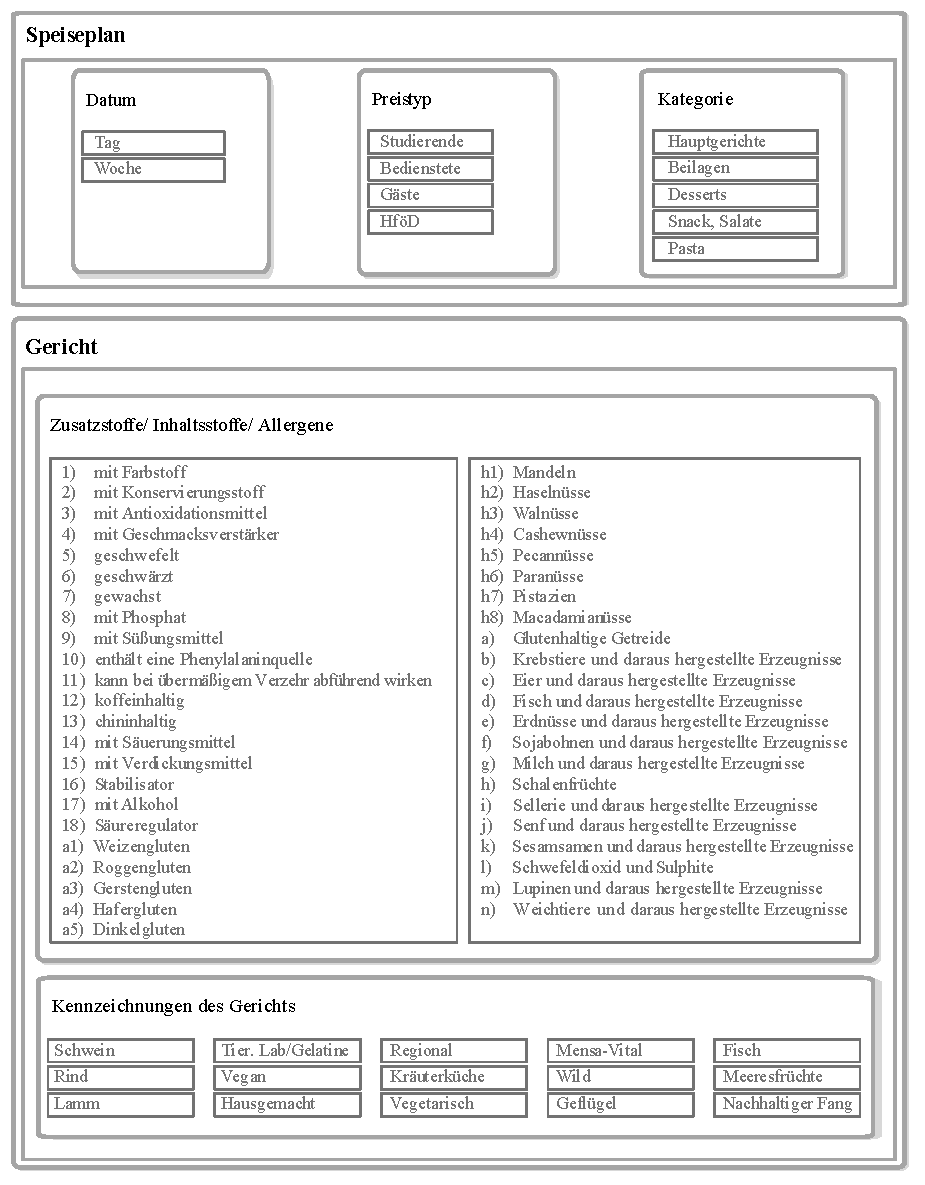
\includegraphics[width=\pictureWidth cm + 2 cm]{Bilder/Sonstiges/Speiseplan_Kategorisierung.pdf}
\caption{Bereiche der Speiseplaninformationen\label{fig:analysemensa}\protect\footnotemark}
\end{figure}\footnotetext{Brysiuk, Lehmann (2019)}




Solange keine Schnittstelle für den Speiseplan zur Verfügung steht, wird ein externer Service erstellt, der die Speiseplan Daten von der Webseite des Stundenwerk-Oberfranken ausliest und in eine Datenbank abspeichert.

% Mensa Umsetzung
\subsection*{Spezifikation der Ressourcen}
\label{sec:mensa_api}
Bezogen auf die technischen Anforderungen aus dem Kapitel \ref{sec:mensa_anforderung} und der Kategorisierung des Speiseplans, werden hier die notwendigen Ressourcen für den Mensa-Service spezifiziert.
\\
\linebreak
Alle GET-Methoden - außer die Subressourcen /filters und /\{id\} - können im Body die Filter für Preis, Kategorie, Kennzeichnung und Zusatzstoffe/Inhaltsstoffe/Allergie der Gerichte entgegen nehmen. Es müssen nicht alle Filter gesetzt werden. Ohne Übergabe der Filter werden standardmäßig alle Gerichte zurückgegeben. Wird der Filter Preistyp gesetzt, so werden nur die Gerichte mit diesem Preistyp zurückgegeben, sonst werden alle Preistypen zurückgegeben. In Kategorie, Zusatzstoffe oder Kennzeichnung des Gerichts können ein oder mehrere Filtertypen festgelegt werden. Wobei die übergebenden Filtertypen für Kategorie und Kennzeichnungen in den Gerichten enthalten sind und die Zusatzstoffe/Inhaltsstoffe/Allergene nicht. 
\begin{itemize}
\item \subsubsection*{GET/POST/DELETE:\\ /menu} 
Die Methode GET liefert alle Gerichte unter der Berücksichtigung von gesetzten Filtern. POST erlaubt erstellen von ein oder mehreren Gerichten und DELETE löscht alle Gerichte. 
\item \subsubsection*{GET/PATCH/DELETE:\\ /menu/\{id\}} 
Die Methode GET liefert ein Gericht für die übergebene ID. Mit PATCH kann das Gericht geändert beziehungsweise korrigiert werden und DELETE löscht dieses Gericht.
\newpage
\item \subsubsection*{GET:\\ /menu/filters} 
Liefert alle Kategorien, Legenden, Zusatzstoffe und Preistypen die vorhanden sind.
\item \subsubsection*{GET/POST/DELETE:\\ /menu/filters/categories} 
Die Methode GET liefert alle möglichen Kategorien. Mit POST können ein oder mehrere neue Kategorien eingefügt werden und DELETE löscht alle verfügbaren Kategorien.
\item \subsubsection*{GET/PATCH/DELETE:\\ /menu/filters/categories/\{id\}} 
Die Methode GET liefert Informationen zur der übergebene Kategorien ID. Mit PATCH kann die Kategorie geändert beziehungsweise korrigiert werden und DELETE löscht diese Kategorie.
\item \subsubsection*{GET/POST/DELETE:\\ /menu/filters/labels} 
Die Methode GET liefert alle möglichen Kennzeichnungen zu den Gerichten. Mit POST können ein oder mehrere neue Kennzeichnungen eingefügt werden und DELETE löscht alle verfügbaren Kennzeichnungen.
\item \subsubsection*{GET/PATCH/DELETE:\\ /menu/filters/labels/\{id\}} 
Die Methode GET liefert Informationen zur der übergebene Kennzeichnung ID. Mit PATCH kann die Kennzeichnung geändert beziehungsweise korrigiert werden und DELETE löscht diese Kennzeichnung.
\newpage
\item \subsubsection*{GET/POST/DELETE:\\ /menu/filters/excludes} 
Die Methode GET liefert alle verfügbaren Zusatzstoffe/Inhaltsstoffe/Allergie. Mit POST können ein oder mehrere neue Zusatzstoffe/Inhaltsstoffe/Allergie eingefügt werden und DELETE löscht alle verfügbaren Zusatzstoffe/Inhaltsstoffe/Allergie. 
\item \subsubsection*{GET/PATCH/DELETE:\\ /menu/filters/excludes/\{id\}} 
Die Methode GET liefert Informationen zur der übergebenen Zusatzstoffe/Inhaltsstoffe/Allergie ID. Mit PATCH kann der Zusatzstoff/Inhaltsstoff/Allergie geändert beziehungsweise korrigiert werden und DELETE löscht diesen Zusatzstoff/Inhaltsstoff/Allergie.
\item \subsubsection*{GET:\\ /menu/filters/prices} 
Die Methode GET liefert alle verfügbaren Preistypen.
\item \subsubsection*{GET:\\ /menu/week} 
Liefert alle Gerichte unter der Berücksichtigung von gesetzten Filtern für die aktuelle Woche.
\item \subsubsection*{GET:\\ /menu/week/\{week\}} 
Liefert alle Gerichte unter der Berücksichtigung von gesetzten Filtern für die übergebene Woche.
\item \subsubsection*{GET:\\ /menu/week/\{week\}/\{day\}} 
Liefert alle Gerichte unter der Berücksichtigung von gesetzten Filtern für den übergebenen Wochentag in der übergebenen Woche.
\item \subsubsection*{GET:\\ /menu/week/\{week\}/\{day\}/\{until-day\}} 
Liefert alle Gerichte unter der Berücksichtigung von gesetzten Filtern für die Zeitspanne innerhalb der übergebenen Wochentagen (inklusiv) in der übergebenen Woche.
\item \subsubsection*{GET:\\ /menu/date} 
Liefert alle Gerichte unter der Berücksichtigung von gesetzten Filtern für den heutigen Tag.
\item \subsubsection*{GET:\\ /menu/date/\{date\}} 
Liefert alle Gerichte unter der Berücksichtigung von gesetzten Filtern für den übergebenden Datum.
\item \subsubsection*{GET:\\ /menu/date/\{date\}/\{until-date\}} 
Liefert alle Gerichte unter der Berücksichtigung von gesetzten Filtern für die Zeitspanne zwischen übergebenen Datumsangaben (inklusiv).
\end{itemize}

% Mensa DB
\subsection*{Datenbank Konzept}
\label{sec:mensa_db}
%Text

Um eine performante und anpassbare Datenquelle für die Daten des Speiseplans des Studentenwerk Oberfrankens zu haben, wird auch hierfür eine Datenbank erstellt. Da sich die Daten kaum ändern entlastet dies auch die Schnittstelle, von der letztendlich die Daten ausgelesen werden. Für die Funktionen des Mensa Services werden lediglich die Gerichte an sich benötigt. Diese Gerichte brauchen folgende Informationen:

\begin{itemize}
\item \textbf{ID} 
\\Einen klaren Identifier für ein Gericht, um für dieses Gericht weitere Informationen abfragen zu können
\item \textbf{Datum} 
\\Das Datum, an dem das Gericht angeboten wird
\item \textbf{Kategorie} 
\\Die Art von Gericht, zu dem der Eintrag zugeteilt werden kann
\item \textbf{Beschreibung} 
\\Eine Kurzbeschreibung für das Gericht
\item \textbf{Zugeordnete Kennzeichnungen} 
\\Kennzeichnungen, die das Gericht beschreiben
\item \textbf{Preis für alle Preistypen} 
\\Verschiedene Preise für verschiedene Gästegruppen
\item \textbf{Enthaltene Zusatzstoffe/Inhaltsstoffe/Allergene} 
\\Hinweise zum Inhalt und für Allergiker
\end{itemize}

Das resultierende \ac{ER}-Diagramm in Abbildung \ref{fig:ermensa} zeigt die einfache Struktur der Datenbank für den Mensa Service. Für die Zusatzstoffe und die Kennzeichner der Gerichte werden sogenannte \textit{n zu n} Beziehungen benötigt, für alles andere reichen Fremdschlüssel zur Zuordnung der weiteren Informationen. Die Tabelle \textit{T_MENU_PRIZE} ähnelt zudem einer Dimensionstabelle eines Data Warehouses, statt die Preise anhand eines Standardwertes berechnen zu müssen, werden alle möglichen Kombinationen abgelegt und können dementsprechend ausgelesen werden. Es bietet sich ebenfalls an, einen \textit{Non-Clustered}-Index auf die Fremdschlüssel zur Tabelle \textit{T_MENU\-_CATEGORY_TYPE} in der Spalte \textit{CATEGORY} der Tabelle \textit{T_MENU_DISH} anzulegen. Des weiteren ist ein weiterer \textit{Non-Clustered}-Index auf der Spalte \textit{DATE} der selben Tabelle sinnvoll. Diese beiden Werte sind die, nach denen am wahrscheinlichsten sortiert und gefiltert wird. Im späteren Betrieb der Datenbank könnte man auch noch testen, ob sich einer der beiden Indizes als \textit{Clustered}-Index eignen würde, da eine dauerhafte Sortierung der Einträge der Tabelle \textit{T_MENU_DISH} nach der \textit{ID} nicht zwingend hilfreich ist.

\begin{figure}[H]
\centering
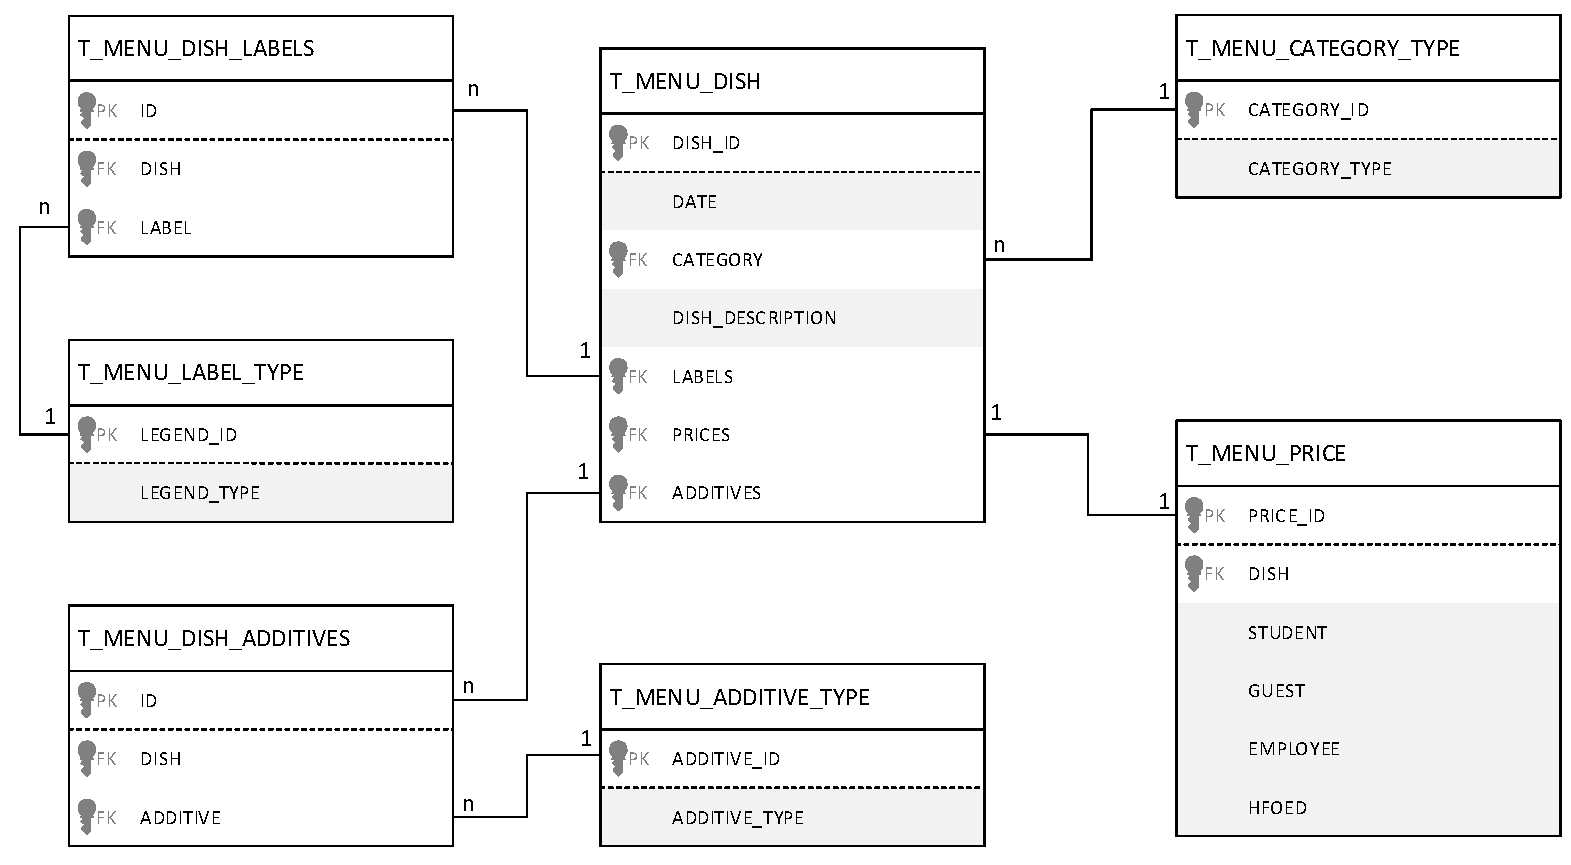
\includegraphics[width=\pictureWidth cm + 2cm]{Bilder/ER/Menu_ER.pdf}
\caption{Entity Relation Digramm des Mensa-Speiseplans\label{fig:ermensa}\protect\footnotemark}
\end{figure}
\footnotetext{Brysiuk, Lehmann (2019)}

Weiterhin zu bemerken ist, dass die Datenbank auf Dauer nur die Gerichte der aktuellen und der nächsten Woche, also im Zeitraum von zwei Wochen, speichern wird. Ein automatisierter Scheduler Job im Mensa Service wird die alten Einträge automatisiert löschen und neue Einträge einspeisen. Für das Löschen der alten Einträge bietet es sich eventuell auch an, einen Datenbank Job zu schreiben, das kann in der Entwicklungsphase getestet werden. Jedoch richtet sich diese Datenbank stark nach dem \ac{KISS} Prinzip, weshalb auch auf komplexere Strukturen verzichtet wurde. Das lässt sich dadurch begründen, dass nur Einträge für den Zeitraum von zwei Wochen gespeichert werden und keine historischen Daten gespeichert werden. Außerdem ist auch eine Änderung in den Formaten der eigentlichen Datenquelle nicht vorhersehbar. Die eigene Tabelle für die Spalte \textit{CATEGORY} der Haupttabelle \textit{T_MENU_DISH} beinhaltet auch eine Beschreibung der einzelnen Einträge, weshalb ein einfacher \textit{Enumeration Type} für diesen Wert keinen Sinn ergibt.


% Notification
\section{Benachrichtigungen (Notification-Service)}
\label{sec:notification}
% Text
Fast in jeder Anwendung sind Push-Notifications eingebunden. Am häufigsten kennt man es von Facebook oder dem Whats-App Messenger, dass die Nachrichten in Echtzeit übertragen werden und direkt auf den Smartphone als Benachrichtigung angezeigt werden. Die Funktionsweise ist einfach, man erhält Benachrichtigungen von einer Programm ohne diese öffnen zu müssen. Dies ermöglichtes, den Benutzer über wichtige Ereignisse oder Neuigkeiten zur informieren ohne die Anwendung zu starten oder diese neu zu laden. Solche Benachrichtigung können für die Studierenden von Vorteil sein. Sollte sich eine Vorlesung ändern oder ausfallen, werden die an der Vorlesung teilnehmenden Studierenden informiert. Aber auch andere Services können von dieser Technik profitieren, wie beispielsweise der Mensa-Service oder der Sprachzentrum-Service. Das Ziel ist es, ein Notification-Service zu erstellen, der eine einheitliche Schnittstelle für alle anderen Services zur Verfügung stellt, um die betroffenen Benutzer über eine Änderung jeglicher Art zu informieren.

\begin{figure}[H]
\centering
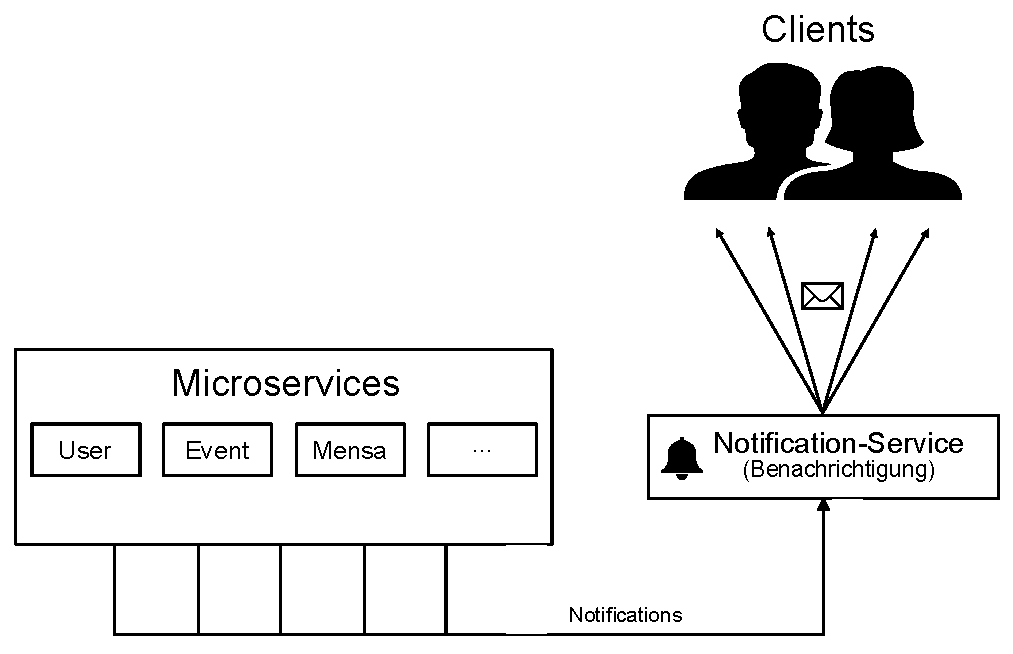
\includegraphics[width=\pictureWidth cm]{Bilder/Prototyp/Notification_Service_Prototype.pdf}
\caption{Benachrichtigungsservice\label{fig:notificationservice}\protect\footnotemark}
\end{figure}
\footnotetext{Brysiuk, Lehmann (2019)}


% Benachrichtigung Anforderung
\subsection*{Anforderung an Schnittstelle}
\label{sec:notification_anforderung}
% Text
Die Funktionalität eines Services, der den Notification-Service in Anspruch nimmt, darf nicht vom Ergebnis des Services beeinflusst werden. Sobald ein Service eine Benachrichtigung an den Notification-Service übermittelt, ist es dem Service nicht mehr wichtig wie, wann und ob die Nachricht zugestellt wird. Damit wird die Abhängigkeit zwischen unterschiedlichen Funktionalitäten reduziert und es wird ein Maß an loser Kopplung garantiert.

\begin{figure}[H]
\centering
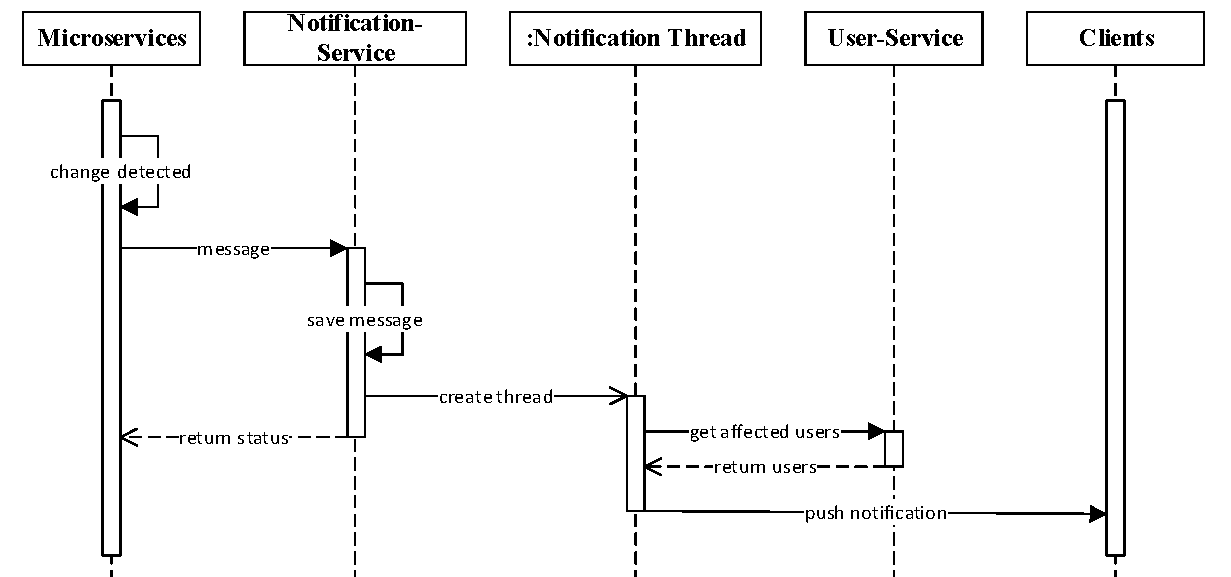
\includegraphics[width=\pictureWidth cm + 2 cm]{Bilder/Sequenz_Diagramm/Notification_Sequenz.pdf}
\caption{Sequenzdiagramm zum Ablauf einer Benachrichtigung\label{fig:notificationsequenz}\protect\footnotemark}
\end{figure}
\footnotetext{Brysiuk, Lehmann (2019)}

In Abbildung \ref{fig:notificationsequenz} ist ein Sequenz Diagramm zu sehen das einen groben Ablauf darstellt, wie eine Benachrichtigung von einem Microservice bis zum Benutzer kommuniziert wird. Der Microservice sendet die Nachricht an den Notification-Service und endet der Prozess für den Microservice. Der \textit{return status} wird vom Microservice ignoriert, sowohl bei einer erfolgreichen Antwort als auch bei einer nicht erfolgreichen Antwort. Der \textit{return status} wurde im Sequenz Diagramm nur aufgenommen, weil eine \ac{REST}-\ac{API} immer eine Antwort zurück senden muss. Ab jetzt ist nur der Notification-Service zuständig für eine erfolgreiche Übermittlung der Nachricht an die Clients. Um sicher zu gehen, dass die Nachricht nicht auf dem Weg verloren geht, bei ersten Versuch nicht erfolgreich an den Client übermittelt werden kann oder beim Absturz des Services verloren geht, wird die Nachricht zuerst in der Datenbank abgelegt. Der Notification-Service ist selbständig verantwortlich dafür, die jeweiligen Benutzer für die Nachricht zu finden und zu informieren. 

% Benachrichtigung API
\subsection*{Spezifikation der Ressourcen}
\label{sec:notification_api}
Der Notification-Service benötigt im Grunde zwei Ressourcen, die eine zur Registrierung eines Clients, die andere für die Übergabe einer Nachricht. Um den Service leichter mit den Hochschul-\ac{App} Services nutzen zu können, wurde der Service um die Subressourcen \textit{/lectures} und \textit{/mensa} erweitert. Außerdem wurde die Benachrichtigung einzelner Benutzer berücksichtigt. Die Übergabe der Informationen an den Notification-Service erfolgt im Body Bereich. 
\begin{itemize}
\item \subsubsection{POST: \\/register} 
Für die Registrierung des Clients, der über Neuigkeiten informiert werden soll.
\item \subsubsection{POST: \\/message} 
Benachrichtigung an alle Benutzer des registrierten Clients.
\item \subsubsection{POST: \\/message/\{userId\}} 
Benachrichtigung an übergebenen Benutzer.
\item \subsubsection{POST: \\/message/lectures} 
Benachrichtigung an Benutzer, die für die Vorlesung hinterlegt sind.
\item \subsubsection{POST: \\/message/mensa} 
Benachrichtigung an Benutzer, die für ein Gericht hinterlegt sind.
\end{itemize}

% Notification DB
\subsection*{Datenbank Konzept}
\label{sec:notification_db}
Wie bereits vorher erwähnt wurde, werden die Nachrichten temporär in der Datenbank abgespeichert und solange behalten, bis die Benachrichtigung tatsächlich die Benutzer erreicht hat. Durch die Spezifikation der Ressourcen ergeben sich folgende Tabellen.

\begin{enumerate}
\item Abspeicherung der Registrierten Clients
\item Benachrichtigung und zugehörige Informationen
\end{enumerate}


\begin{figure}[H]
\centering
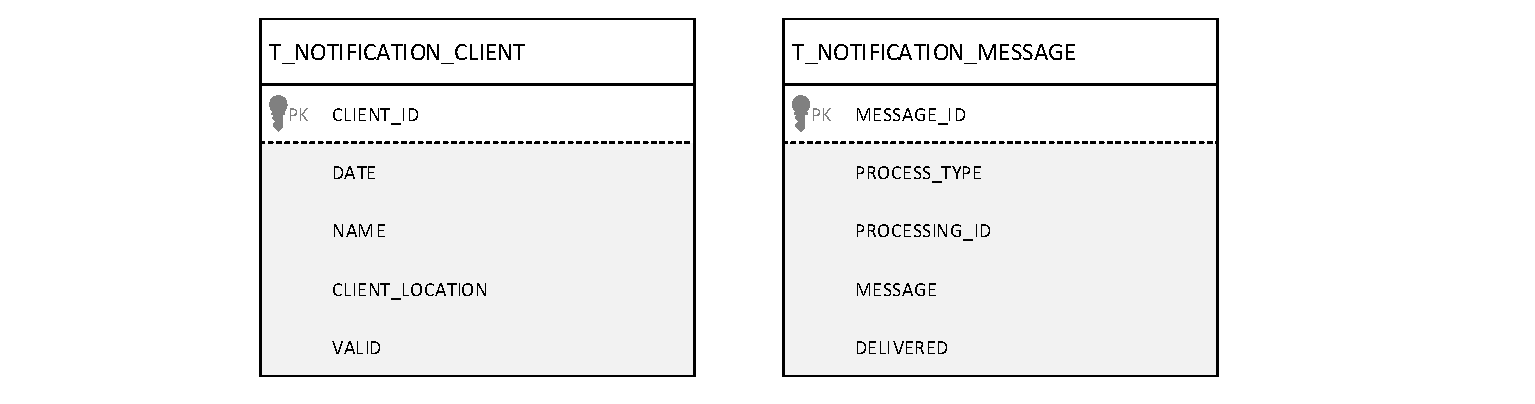
\includegraphics[width=\pictureWidth cm + 3 cm]{Bilder/ER/Notification_ER.pdf}
\caption{Entity Relation Diagramm der Benachrichtigungs Datenbank\label{fig:notificationER}\protect\footnotemark}
\end{figure}
\footnotetext{Brysiuk, Lehmann (2019)}


% Auth
\section{Sicherheit (Auth-Service)}
\label{sec:auth}
% Text
Um alle Services abzusichern, wird ein Sicherheitskonzept benötigt. Zum einen müssen die Clients autorisiert werden und anderen die Benutzer authentifiziert werden. Um einen gesicherten Zugriff auf die Microservices zu gewährleisten, ohne dass die Services vom Authentifizierung-Service abhängig sind, wird ein Token an die Microservices übersendet, über welchen die Zugriffserlaubnis von jeden Service unabhängig geprüft werden kann, ohne den Authentifizierung Service aufzurufen.

\begin{figure}[H]
\centering
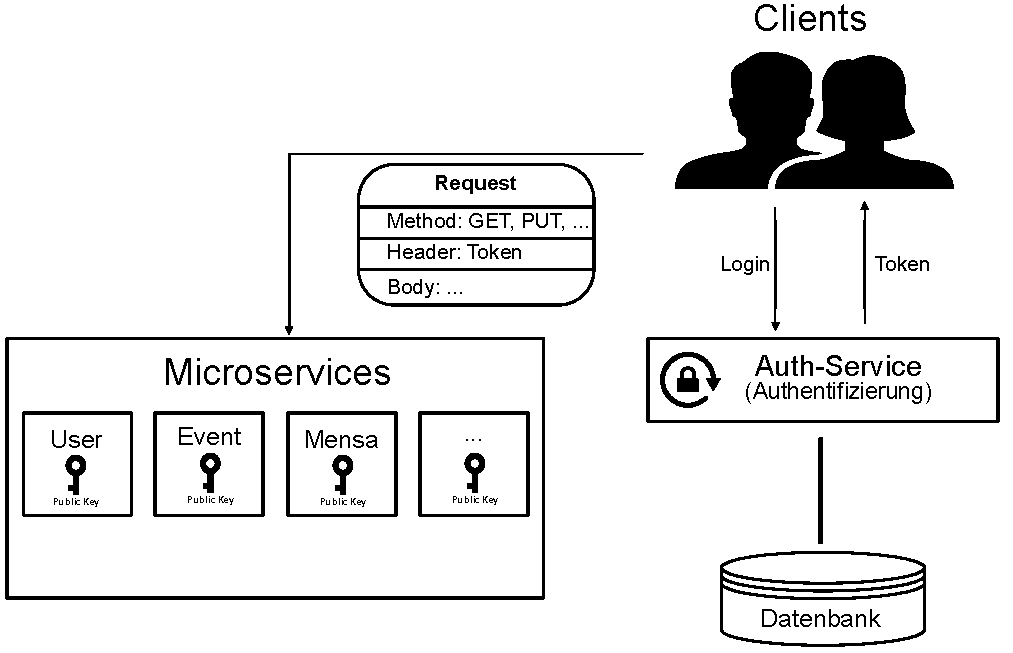
\includegraphics[width=\pictureWidth cm]{Bilder/Prototyp/Auth_Service_Prototype.pdf}
\caption{Authentifizierungsservice\label{fig:authservice}\protect\footnotemark}
\end{figure}
\footnotetext{ebd.}

Für die Zugriffssteuerung wird das Konzept von Rollen und Rechten verwendet. Ausführliche Behandlung diesen Services ist in der hierzu parallel angefertigten Bachelorarbeit zu sehen\autocite[Vgl.][]{andreasba}.

% user
\section{Anwenderverwaltung (User-Service)}
\label{sec:user}
%Text
Der User-Service dient dazu, Benutzer zu verwalten und das mitsamt ihrer Accountinformationen und Einstellungen. Die ausführliche Behandlung dieses Services ist in der hierzu parallel angefertigten Bachelorarbeit zu sehen\footnote{ebd.}.

% Futher Information
\section{Weitere Dienste}
\label{sec:ausblick}
%Text
Die Services Sprachzentrum und Termine sind zwar in der Architektur der Hoch\-schul-\ac{App} berücksichtigt worden, jedoch überschreiten diese den Umfang dieser Bachelorarbeit. Durch die modularisierte und flexible Architektur können diese Services jederzeit separat entwickelt werden und an die aus dieser Arbeit entstandene Hoch\-schul-\ac{App} verknüpft werden.
